\documentclass[english]{socg-lipics-v2021}
\usepackage{pythonhighlight}
\EventEditors{Wolfgang Mulzer and Jeff M. Phillips}
\EventNoEds{2}
\EventLongTitle{40th International Symposium on Computational Geometry
(SoCG 2024)}
\EventShortTitle{SoCG 2024}
\EventAcronym{SoCG}
\EventYear{2024}
\EventDate{June 11-14, 2024}
\EventLocation{Athens, Greece}
\EventLogo{socg-logo.pdf}
\SeriesVolume{293}
\ArticleNo{XX}     % <-- This will be filled in by the typesetters

\category{Media Exposition}

\title{Visualizing Lucas's Hamiltonian Paths Through The Associahedron 1-Skeleton}

\author{Kacey Thien-Huu La}{Ursinus College Mathematics And Computer Science, Collegeville, PA, USA }{}{}{}
\author{Jose E. Arbelo}{Ursinus College Mathematics And Computer Science, Collegeville, PA, USA }{}{}{}
\author{Christopher J. Tralie}{Ursinus College Mathematics And Computer Science, Collegeville, PA, USA \url{https://www.ctralie.com} }{ctralie@alumni.princeton.edu}{https://orcid.org/0000-0003-4206-1963}{}

\authorrunning{K.T.H La, J.E. Arbelo, C.J. Tralie}
\Copyright{Christopher J. Tralie}
\titlerunning{Visualizing Lucas's Hamiltonian Associahedron}
\ccsdesc{Human-centered computing~Visualization toolkits}
\ccsdesc{Theory of computation~Randomness, geometry and discrete structures}
\keywords{associahedron, hamiltonian paths, visualization, tree rotations, convex polygons}


\supplementdetails[subcategory={Source Code}]{Software}{https://associahedron.github.io/viz/}


\begin{document}
\maketitle
\begin{abstract}
    
We re-examine the 1987 paper by Joan Lucas\cite{lucas1987rotation}, who showed that the edge-flip graph of convex polygon triangulations is Hamiltonian.  We focus specifically on the first part of her paper on Hamiltonian paths, and we provide a simplified algorithm for that case which elucidates how to assemble a recursive subdivision that she refers to as ``stacks.''  Finally, we provide an interactive web-based visualization of Hamiltonian paths through the stacks.

\end{abstract}

\begin{figure}
    \centering
    \includegraphics[width=0.8\textwidth]{a4.pdf}
    \caption{The flip graph is the 1-skeleton of the associahedron.  Edges are between triangulations that differ by a single edge flip.  In the above, a Hamiltonian path (pink) is shown through all hexagon triangulations in $K_4$, a 3D polytope. We superimpose Lucas's codewords on each triangulation.}
    \label{fig:associahedron}
\end{figure}

\begin{figure}
    \centering
    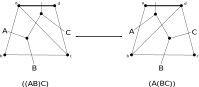
\includegraphics[width=0.8\textwidth]{correspondences.pdf}
    \caption{Vertices of the flip graph correspond to triangulations of $n+2$-gons, but also to binary trees with $n$ internal nodes and balanced parentheses on $n+1$ items.  Edges are between convex polygons with a quad edge flip, trees with a rotation between them, or parentheses with a single re-association, respectively.}
    \label{fig:correspondences}
\end{figure}



\section{Convex Flip Graphs}

A \textbf{flip graph} for the triangulation of a particular polygon has a vertex for each possible triangulation, and an edge between two vertices if their corresponding triangulations differ by a single \textbf{quadrilateral edge flip}.  In the special case of convex polygon with $n+2$ vertices and a designated top edge, the flip graph can be realized as the 1-skeleton of a convex polytope known as the \textbf{associahedron $K_n$} (Figure~\ref{fig:associahedron}).  This polytope has ``Catalan number'' $C_n = \frac{1}{n+1} \binom{2n}{n}$ vertices, each of whose $i^{\text{th}}$ coordinate in $\mathbb{R}^{n+2}$ is the total area of all triangles adjacent to vertex $i$ \footnote{Though this is in $n+2$ dimensions, the geometry can be isometrically embedded in $n-1$ dimensions.}.  Since there is a bijection between the triangulations and all possible rooted binary search trees with $n$ internal nodes and $n+1$ leaf nodes, the flip graph is also called the ``rotation graph''  \cite{lucas1987rotation}.  In this context, an edge in $K_n$ corresponds to a single {\bf tree rotation} (Figure~\ref{fig:correspondences}).  Among many other ``Catalan bijections'' \cite{roman2015introduction}, there is also a bijection with all balanced parentheses on $n+1$ items, where an edge is a single re-association.

\section{Enumerating And Visualizing A Hamiltonian Path}


\begin{figure}
    \centering
    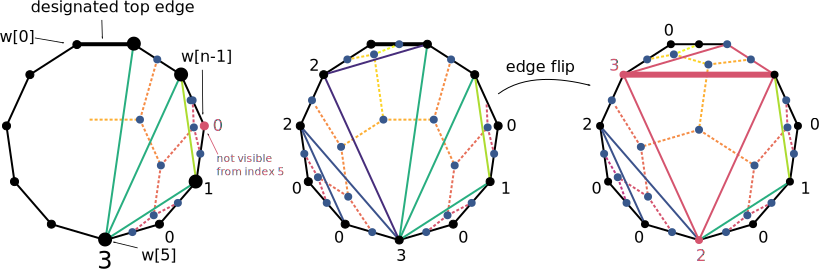
\includegraphics[width=\textwidth]{elevengon.pdf}
    \caption{Construct a triangulation from a valid codeword starting at the end and working back in a counter-clockwise fashion, adding $w[i]$ edges to the closest visible vertices at $j > i+1$.  Upon completion, extract the corresponding binary tree by putting an internal node in each triangle and connecting nodes belonging to adjacent triangles.  Leaf nodes are on the boundary edges of the polygon.  An edge flip in a quad decrements one entry of $w$ and increments another.}
    \label{fig:construct}
\end{figure}

Remarkably, as Joan Lucas shows in her 1987 paper \cite{lucas1987rotation}, the flip graph is Hamiltonian.  To show this, she uses \textbf{codeword encodings} of triangulations introduced by Zerling \cite{zerling1985generating} to design an $O(C_n)$ time algorithm for enumerating Hamiltonian paths and cycles.  Specifically, the $i^{\text{th}}$ entry of a codeword $w$ counts the number of internal edges incident on vertex $i$ that connect to a vertex with a greater index, where $w[0]$ corresponds to the left of the top edge.  As such, each internal edge contributes to exactly one entry.  As Lucas proves \cite{lucas1987rotation}, a codeword is a \textbf{valid codeword} of a convex polygon triangulation if and only if:
\begin{equation}
    \label{eq:valid1}
    \sum_{i=0}^{n-1} w[i] = n-1
\end{equation}
and
\begin{equation}
    \label{eq:valid2}
    w[i] \leq n - i - \sum_{k=i+1}^{n-1} w[k], 0 < i < n
\end{equation}



The first condition follows since triangulations of polygons with $n+2$ vertices have exactly $n-1$ internal edges, and the second condition prevents internal edge crossings.   Given a valid codeword, one can construct the corresponding triangulation by starting at vertex $i-1$ and moving backwards one vertex at a time to vertex $0$, adding $w[i]$ internal edges at each step to the closest visible vertices with indices $> i+1$ (Figure~\ref{fig:construct}).

\begin{figure}
    \centering
    \includegraphics[width=\textwidth]{RotationExamples.pdf}
    \caption{All of the above examples increment one entry and decrement a different entry to move from $w_1$ to $w_2$, but not all describe a single valid edge flip in a quadrilateral.}
    \label{fig:rotexamples}
\end{figure}


A necessary condition for a single edge flip between codewords $w_1$ and $w_2$ is

\begin{equation}
    \label{eq:rot1}
    w_1[a] = w_2[b] \pm 1, w_2[b] = w_1[a] \mp 1, a < b \text{, and }  w_1[k] = w_2[k], k \notin \{a, b\}
\end{equation}

Intuitively, the vertices at indices $a, b$ are the base of a quadrilateral where an edge flip happens, and they exchange exactly one edge.  However, this is not sufficient; the quad should also be free of other internal edges, and the polygonal region below $ab$ should be fully triangulated.  Formally, the following two additional conditions are sufficient (\cite{lucas1987rotation} Lemma 2):

\begin{equation}
    \label{eq:rot2}
    \sum_{\ell = k}^{b-1}  w_1[\ell] < b-k, a < k < b
\end{equation}

\begin{equation}
    \label{eq:rot3}
    \sum_{\ell = a}^{b-1} w_1[\ell] \geq (b - a) + \delta_{w_1[a]+1, w_2[a]} - \delta_{a,0} \text{,  where }  \delta_{x,y} = \left\{ \begin{array}{cc} 1 & x = y \\ 0 & x \neq y \end{array} \right\}
\end{equation}

The first Kronecker $\delta$ case accounts for an edge flip moving a diagonal out of $a$, and the second $\delta$ accounts for the top boundary edge which may be edge $ad$ of the quad $abcd$.



A codeword $w$ is in {\bf $d$-extreme}, $1 \leq d \leq n-1$, if $w[i] = 0$ or $w[i] = n-i-\sum_{k=i+1}^{n-1} w[k]$ for all $1 \leq i \leq d$.  Lucas proves that if an edge flip is possible using index $d+1$ in a $d$-extreme codeword $w_1$, then the resulting codeword $w_2$ is also $d$-extreme (Figure~\ref{fig:extreme}, Lemma 3 in \cite{lucas1987rotation}).

\begin{figure}
    \centering
    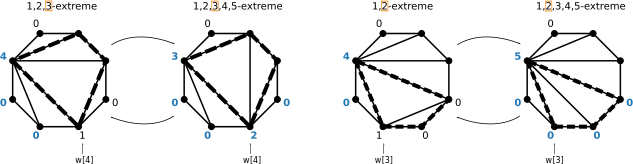
\includegraphics[width=\textwidth]{Extreme.pdf}
    \caption{A $d$-extreme codeword remains $d$-extreme after an edge flip involving index $d+1$.}
    \label{fig:extreme}
\end{figure}


Finally, Lucas defines a {\bf $d$-dimensional stack} as the set of valid codewords that share the last $n-d-1$ entries.  ``Dimension'' is apt here, as such a codeword has $d$ degrees of freedom; there are $d+1$ unspecified entries, but $w[0]$ is linearly dependent on the rest given Equation~\ref{eq:valid1}.  Furthermore, define the {\bf height $h$ of a stack} as the number of possible entries $w[d]$ can take on in a particular $d$-dimensional stack $S$.  Based on Equation~\ref{eq:valid2}, this is

\begin{equation}
    h = \left(n-d-\sum_{k=d+1}^{n-1} w[k]\right) + 1
\end{equation}


\begin{figure}
    \begin{python}
def make_stack_rec(w, d, stack_index, wsum): 
    n = len(w)
    h = n-d-wsum+1 # where wsum = sum(w[d+1:])
    vals = list(range(h)) # Entry in w[d] for each substack
    if stack_index[d]%2 == 1: # Reverse every other d-dim substack
        vals = reversed(vals)
    stack_index[d] += 1
    for val in vals:
        w[d] = val
        if d == 1: ## Base case
            w[0] = n-1-(w[d]+wsum) # Equation 1 re-arranged
            print(w) # This will print the codewords in Hamiltonian order
        else:
            make_stack_rec(w, d-1, stack_index, wsum+val)
def print_hamiltonian(n): # Print a Hamiltonian traversal of Kn
    make_stack_rec([0]*n, n-1, [0]*n, 0) # Start on an (n-1)-extreme node
        \end{python}
    \caption{A simplified $O(C_n)$ algorithm to enumerate a Hamiltonian path through $K_n$.}
    \label{fig:algorithm}
\end{figure}

Lucas shows by induction that, given a $d$-extreme codeword $w$ in a stack $S$ of height $h$, it's possible to find a Hamiltonian path through $S$ that starts on $w$ and ends on another $d$-extreme codeword (Theorem 1 in \cite{lucas1987rotation}). The base case $d=1$ is trivial, as it is a simple 1D path.  For $d > 1$, one can partition $S$ into $h$ {\bf substacks} $\{S(i) = \{w \in S | w[d] = i\} \}_{i=0}^{h-1}$.  Assuming by induction that each substack begins and ends on a $d-1$-extreme codeword, arrange the substacks in either ascending or descending order by $i$ to assemble them into a Hamiltonian path through all of $S$.  To ensure that the boundary of adjacent substacks differ by a single edge flip, \textbf{assemble adjacent substacks in reverse order of each other}.  

The above can be used to construct a Hamiltonian path through the entire edge flip graph, which is an $n-1$ dimensional stack of height $2$, starting on the codeword $w = [n-1, 0, ..., 0]$.  We show a complete implementation as recursive python code in Figure~\ref{fig:algorithm}, which is slightly simpler than Lucas's provided code.  Figure~\ref{fig:stacks} shows this assembly visually for $n=2,3,4$, where substacks that are presented in reverse order by $i$ are highlighted in gray.  We believe it is easier to visualize the Hamiltonian path unraveled in this way than it is to superimpose it on the associahedron itself (as in Figure~\ref{fig:associahedron}), particularly in higher dimensions.  To help make this even clearer, we also provide a Javascript web app using d3 \cite{bostock2011d3} to animate the Hamiltonian path one step at a time, which we trace through the substacks.



\begin{figure}
    \centering
    \includegraphics[width=\textwidth]{stacks.pdf}
    \caption{All stacks for $n=2,3,4$ laid out vertically in Hamiltonian order by the algorithm in Figure~\ref{fig:algorithm}.  Flipped edges from adjacent polygons in order are depicted as dashed lines, with changed codeword indices circled.  Every other substack is presented in the reverse order (gray) so they fit together at adjacent extreme codewords.}
    \label{fig:stacks}
\end{figure}


\bibliographystyle{plainurl}
\bibliography{main}

\end{document}